% color definitions

\documentclass[multi=tikzpicture,varwidth=true, border=5mm]{standalone}
\usepackage{tikz}
\usepackage{xcolor}

\begin{document}
% % % % % GROUP 1 - 5
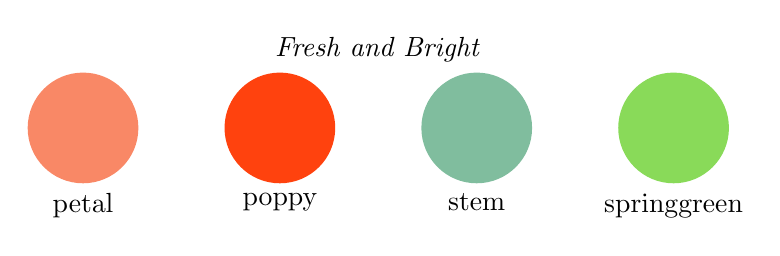
\begin{tikzpicture}[mynode/.style={circle,minimum size=40}]
\definecolor{petal}{HTML}{F98866}
\definecolor{poppy}{HTML}{FF420E}
\definecolor{stem}{HTML}{80BD9E}
\definecolor{springgreen}{HTML}{89DA59}
  \foreach \crlr/\pos in {petal/1,poppy/2,stem/3,springgreen/4}
  {  \node [mynode,fill=\crlr,label=below:\crlr] () at (2.5*\pos,0) {};}
\node at (6.25, 1) {\textit{Fresh and Bright}};
\end{tikzpicture}

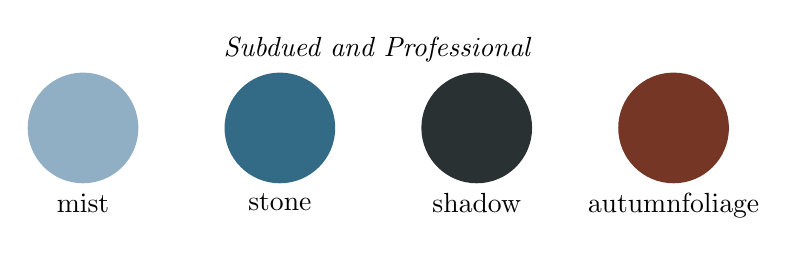
\begin{tikzpicture}[mynode/.style={circle,minimum size=40}]
\definecolor{mist}{HTML}{90AFC5}
\definecolor{stone}{HTML}{336B87}
\definecolor{shadow}{HTML}{2A3132}
\definecolor{autumnfoliage}{HTML}{763626}
  \foreach \crlr/\pos in {mist/1,stone/2,shadow/3,autumnfoliage/4}
  {  \node [mynode,fill=\crlr,label=below:\crlr] () at (2.5*\pos,0) {};}
\node at (6.25, 1) {\textit{Subdued and Professional}};
\end{tikzpicture}

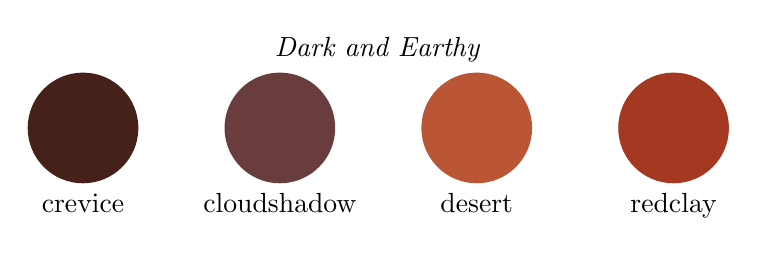
\begin{tikzpicture}[mynode/.style={circle,minimum size=40}]
\definecolor{crevice}{HTML}{46211A}
\definecolor{cloudshadow}{HTML}{693D3D}
\definecolor{desert}{HTML}{BA5536}
\definecolor{redclay}{HTML}{A43820}
  \foreach \crlr/\pos in {crevice/1,cloudshadow/2,desert/3,redclay/4}
  {  \node [mynode,fill=\crlr,label=below:\crlr] () at (2.5*\pos,0) {};}
\node at (6.25, 1) {\textit{Dark and Earthy}};
\end{tikzpicture}

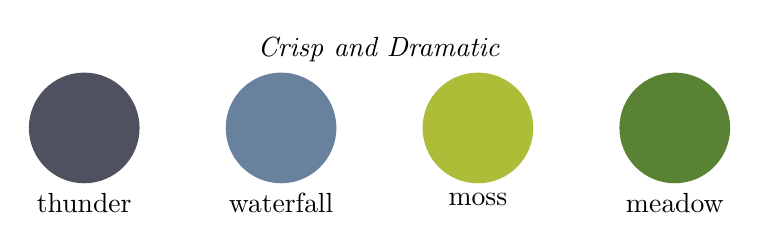
\begin{tikzpicture}[mynode/.style={circle,minimum size=40}]
\definecolor{thunder}{HTML}{505160}
\definecolor{waterfall}{HTML}{68829E}
\definecolor{moss}{HTML}{AEBD38}
\definecolor{meadow}{HTML}{598234}
  \foreach \crlr/\pos in {thunder/1,waterfall/2,moss/3,meadow/4}
  {  \node [mynode,fill=\crlr,label=below:\crlr] () at (2.5*\pos,0) {};}
\node at (6.25, 1) {\textit{Crisp and Dramatic}};
\end{tikzpicture}

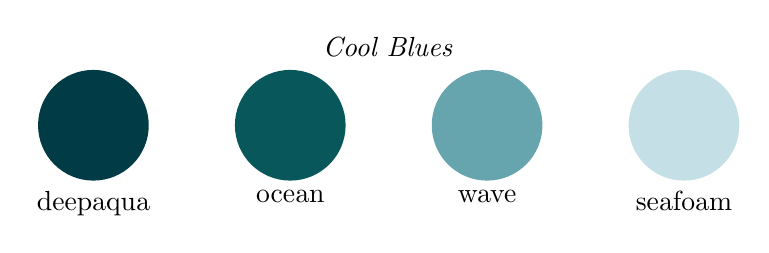
\begin{tikzpicture}[mynode/.style={circle,minimum size=40}]
\definecolor{deepaqua}{HTML}{003B46}
\definecolor{ocean}{HTML}{07575B}
\definecolor{wave}{HTML}{66A5AD}
\definecolor{seafoam}{HTML}{C4DFE6}
  \foreach \crlr/\pos in {deepaqua/1,ocean/2,wave/3,seafoam/4}
  {  \node [mynode,fill=\crlr,label=below:\crlr] () at (2.5*\pos,0) {};}
\node at (6.25, 1) {\textit{Cool Blues}};
\end{tikzpicture}

% % % % % GROUP 6 - 10
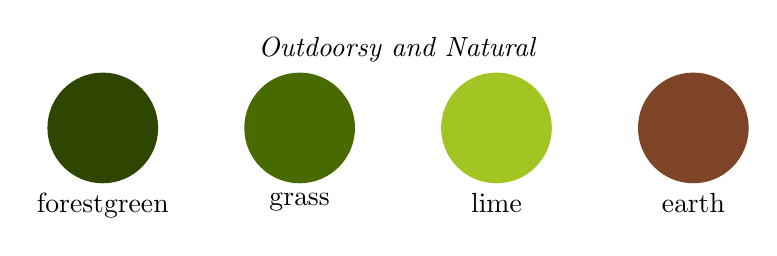
\begin{tikzpicture}[mynode/.style={circle,minimum size=40}]
\definecolor{forestgreen}{HTML}{2E4600}
\definecolor{grass}{HTML}{486B00}
\definecolor{lime}{HTML}{A2C523}
\definecolor{earth}{HTML}{7D4427}
  \foreach \crlr/\pos in {forestgreen/1,grass/2,lime/3,earth/4}
  {  \node [mynode,fill=\crlr,label=below:\crlr] () at (2.5*\pos,0) {};}
\node at (6.25, 1) {\textit{Outdoorsy and Natural}};
\end{tikzpicture}

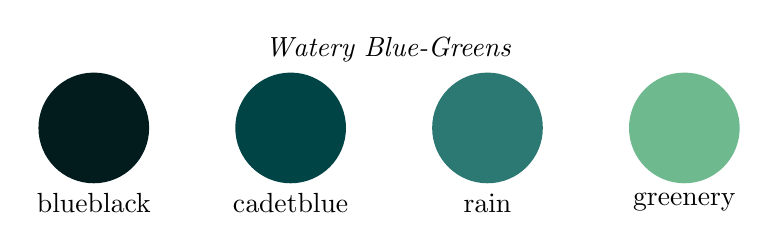
\begin{tikzpicture}[mynode/.style={circle,minimum size=40}]
\definecolor{blueblack}{HTML}{021C1E}
\definecolor{cadetblue}{HTML}{004445}
\definecolor{rain}{HTML}{2C7873}
\definecolor{greenery}{HTML}{6FB98F}
  \foreach \crlr/\pos in {blueblack/1,cadetblue/2,rain/3,greenery/4}
  {  \node [mynode,fill=\crlr,label=below:\crlr] () at (2.5*\pos,0) {};}
\node at (6.25, 1) {\textit{Watery Blue-Greens}};
\end{tikzpicture}

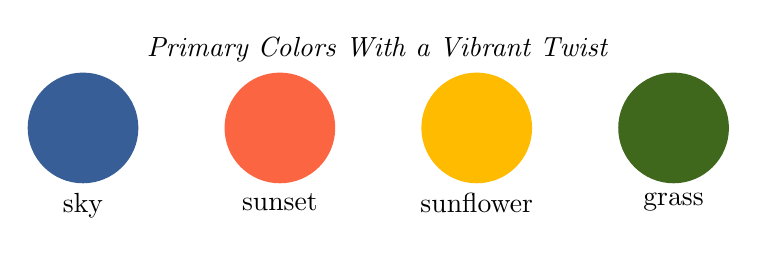
\begin{tikzpicture}[mynode/.style={circle,minimum size=40}]
\definecolor{sky}{HTML}{375E97}
\definecolor{sunset}{HTML}{FB6542}
\definecolor{sunflower}{HTML}{FFBB00}
\definecolor{grass}{HTML}{3F681C}
  \foreach \crlr/\pos in {sky/1,sunset/2,sunflower/3,grass/4}
  {  \node [mynode,fill=\crlr,label=below:\crlr] () at (2.5*\pos,0) {};}
\node at (6.25, 1) {\textit{Primary Colors With a Vibrant Twist}};
\end{tikzpicture}

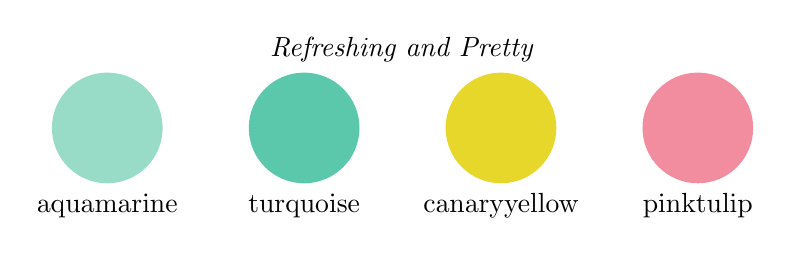
\begin{tikzpicture}[mynode/.style={circle,minimum size=40}]
\definecolor{aquamarine}{HTML}{98DBC6}
\definecolor{turquoise}{HTML}{5BC8AC}
\definecolor{canaryyellow}{HTML}{E6D72A}
\definecolor{pinktulip}{HTML}{F18D9E}
  \foreach \crlr/\pos in {aquamarine/1,turquoise/2,canaryyellow/3,pinktulip/4}
  {  \node [mynode,fill=\crlr,label=below:\crlr] () at (2.5*\pos,0) {};}
\node at (6.25, 1) {\textit{Refreshing and Pretty}};
\end{tikzpicture}

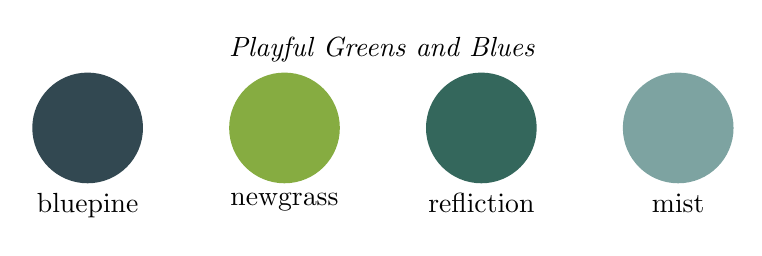
\begin{tikzpicture}[mynode/.style={circle,minimum size=40}]
\definecolor{bluepine}{HTML}{324851}
\definecolor{newgrass}{HTML}{86AC41}
\definecolor{refliction}{HTML}{34675C}
\definecolor{mist}{HTML}{7DA3A1}
  \foreach \crlr/\pos in {bluepine/1,newgrass/2,refliction/3,mist/4}
  {  \node [mynode,fill=\crlr,label=below:\crlr] () at (2.5*\pos,0) {};}
\node at (6.25, 1) {\textit{Playful Greens and Blues}};
\end{tikzpicture}

% % % % % GROUP 11 - 15
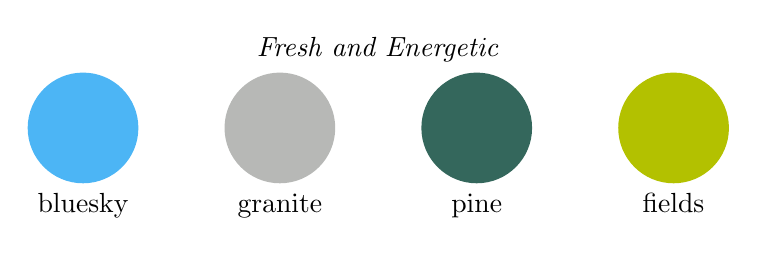
\begin{tikzpicture}[mynode/.style={circle,minimum size=40}]
\definecolor{bluesky}{HTML}{4CB5F5}
\definecolor{granite}{HTML}{B7B8B6}
\definecolor{pine}{HTML}{34675C}
\definecolor{fields}{HTML}{B3C100}
  \foreach \crlr/\pos in {bluesky/1,granite/2,pine/3,fields/4}
  {  \node [mynode,fill=\crlr,label=below:\crlr] () at (2.5*\pos,0) {};}
\node at (6.25, 1) {\textit{Fresh and Energetic}};
\end{tikzpicture}

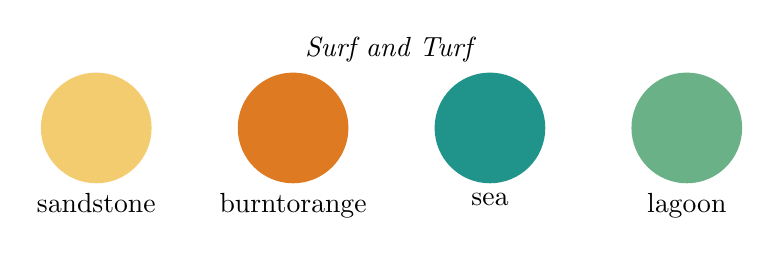
\begin{tikzpicture}[mynode/.style={circle,minimum size=40}]
\node at (6.25, 1) {\textit{Surf and Turf}};
\definecolor{sandstone}{HTML}{F4CC70}
\definecolor{burntorange}{HTML}{DE7A22}
\definecolor{sea}{HTML}{20948B}
\definecolor{lagoon}{HTML}{6AB187}
  \foreach \crlr/\pos in {sandstone/1,burntorange/2,sea/3,lagoon/4}
  {  \node [mynode,fill=\crlr,label=below:\crlr] () at (2.5*\pos,0) {};}
\end{tikzpicture}

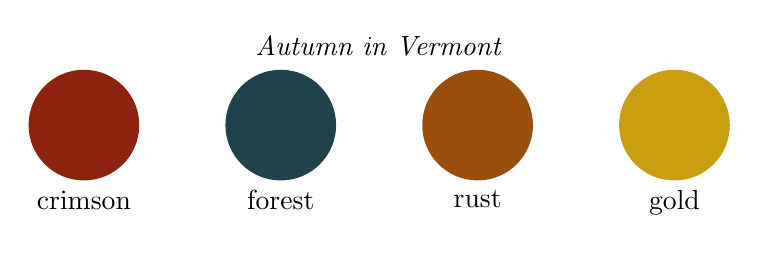
\begin{tikzpicture}[mynode/.style={circle,minimum size=40}]
\node at (6.25, 1) {\textit{Autumn in Vermont}};
\definecolor{crimson}{HTML}{8D230F}
\definecolor{forest}{HTML}{1E434C}
\definecolor{rust}{HTML}{9B4F0F}
\definecolor{gold}{HTML}{C99E10}
  \foreach \crlr/\pos in {crimson/1,forest/2,rust/3,gold/4}
  {  \node [mynode,fill=\crlr,label=below:\crlr] () at (2.5*\pos,0) {};}
\end{tikzpicture}

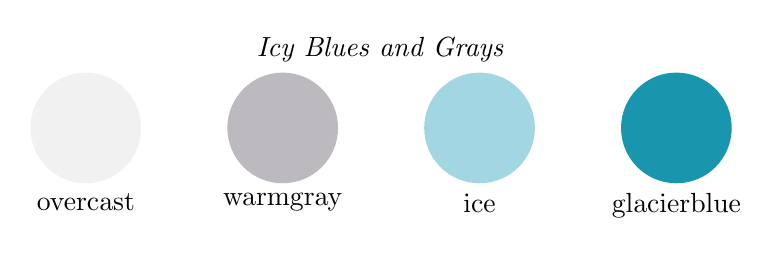
\begin{tikzpicture}[mynode/.style={circle,minimum size=40}]
\node at (6.25, 1) {\textit{Icy Blues and Grays}};
\definecolor{overcast}{HTML}{F1F1F2}
\definecolor{warmgray}{HTML}{BCBABE}
\definecolor{ice}{HTML}{A1D6E2}
\definecolor{glacierblue}{HTML}{1995AD}
  \foreach \crlr/\pos in {overcast/1,warmgray/2,ice/3,glacierblue/4}
  {  \node [mynode,fill=\crlr,label=below:\crlr] () at (2.5*\pos,0) {};}
\end{tikzpicture}


\begin{tikzpicture}[mynode/.style={circle,minimum size=40}]
\node at (6.25, 1) {\textit{Birds and Berries}};
\definecolor{lavendergray}{HTML}{9A9EAB}
\definecolor{branch}{HTML}{5D535E}
\definecolor{berry}{HTML}{EC96A4}
\definecolor{yellowfeathers}{HTML}{DFE166}
  \foreach \crlr/\pos in {lavendergray/1,branch/2,berry/3,yellowfeathers/4}
  {  \node [mynode,fill=\crlr,label=below:\crlr] () at (2.5*\pos,0) {};}
\end{tikzpicture}

% % % % % GROUP 16 - 20
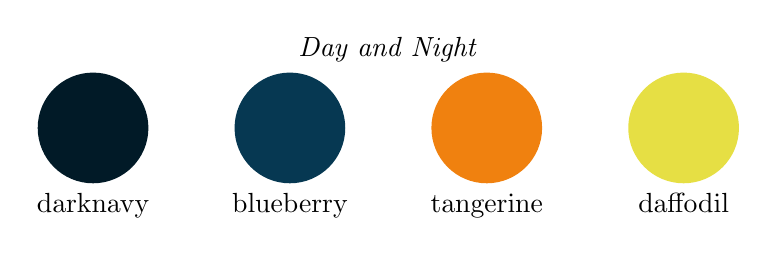
\begin{tikzpicture}[mynode/.style={circle,minimum size=40}]
\node at (6.25, 1) {\textit{Day and Night}};
\definecolor{darknavy}{HTML}{011A27}
\definecolor{blueberry}{HTML}{063852}
\definecolor{tangerine}{HTML}{F0810F}
\definecolor{daffodil}{HTML}{E6DF44}
  \foreach \crlr/\pos in {darknavy/1,blueberry/2,tangerine/3,daffodil/4}
  {  \node [mynode,fill=\crlr,label=below:\crlr] () at (2.5*\pos,0) {};}
\end{tikzpicture}

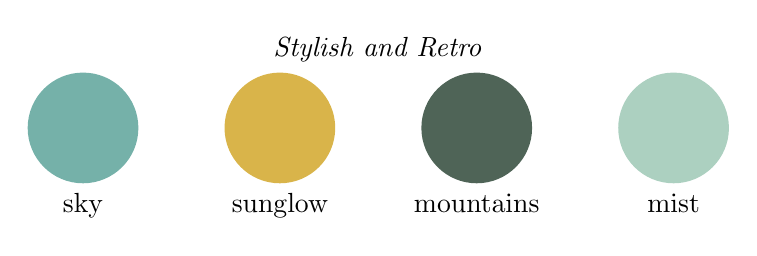
\begin{tikzpicture}[mynode/.style={circle,minimum size=40}]
\node at (6.25, 1) {\textit{Stylish and Retro}};
\definecolor{sky}{HTML}{75B1A9}
\definecolor{sunglow}{HTML}{D9B44A}
\definecolor{mountains}{HTML}{4F6457}
\definecolor{mist}{HTML}{ACD0C0}
  \foreach \crlr/\pos in {sky/1,sunglow/2,mountains/3,mist/4}
  {  \node [mynode,fill=\crlr,label=below:\crlr] () at (2.5*\pos,0) {};}
\end{tikzpicture}

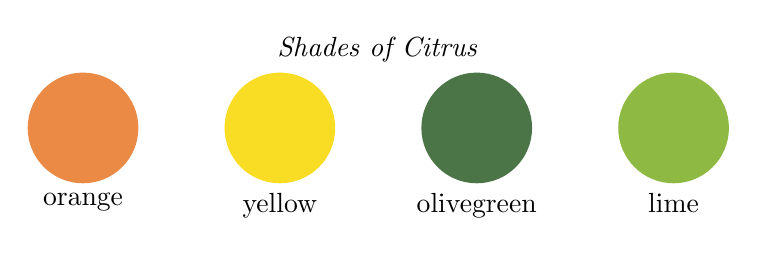
\begin{tikzpicture}[mynode/.style={circle,minimum size=40}]
\node at (6.25, 1) {\textit{Shades of Citrus}};
\definecolor{orange}{HTML}{EB8A44}
\definecolor{yellow}{HTML}{F9DC24}
\definecolor{olivegreen}{HTML}{4B7447}
\definecolor{lime}{HTML}{8EBA43}
  \foreach \crlr/\pos in {orange/1,yellow/2,olivegreen/3,lime/4}
  {  \node [mynode,fill=\crlr,label=below:\crlr] () at (2.5*\pos,0) {};}
\end{tikzpicture}

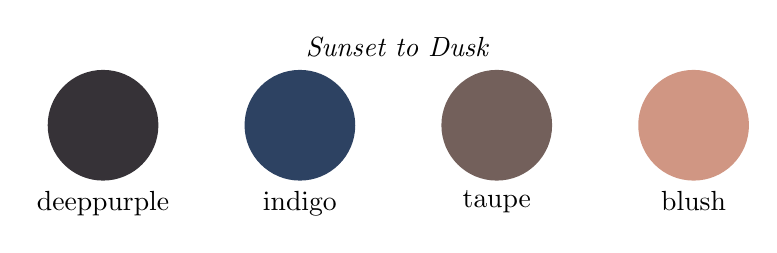
\begin{tikzpicture}[mynode/.style={circle,minimum size=40}]
\node at (6.25, 1) {\textit{Sunset to Dusk}};
\definecolor{deeppurple}{HTML}{363237}
\definecolor{indigo}{HTML}{2D4262}
\definecolor{taupe}{HTML}{73605B}
\definecolor{blush}{HTML}{D09683}
  \foreach \crlr/\pos in {deeppurple/1,indigo/2,taupe/3,blush/4}
  {  \node [mynode,fill=\crlr,label=below:\crlr] () at (2.5*\pos,0) {};}
\end{tikzpicture}

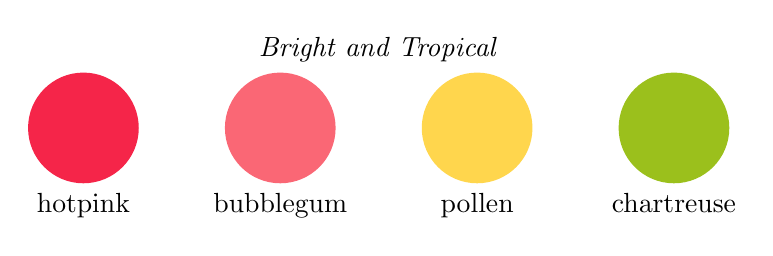
\begin{tikzpicture}[mynode/.style={circle,minimum size=40}]
\node at (6.25, 1) {\textit{Bright and Tropical}};
\definecolor{hotpink}{HTML}{F52549}
\definecolor{bubblegum}{HTML}{FA6775}
\definecolor{pollen}{HTML}{FFD64D}
\definecolor{chartreuse}{HTML}{9BC01C}
  \foreach \crlr/\pos in {hotpink/1,bubblegum/2,pollen/3,chartreuse/4}
  {  \node [mynode,fill=\crlr,label=below:\crlr] () at (2.5*\pos,0) {};}
\end{tikzpicture}

% % % % % GROUP 21 - 25
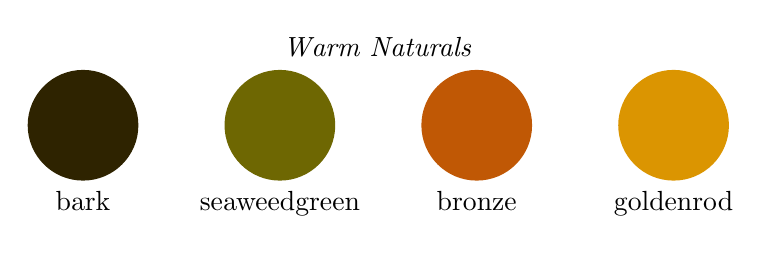
\begin{tikzpicture}[mynode/.style={circle,minimum size=40}]
\node at (6.25, 1) {\textit{Warm Naturals}};
\definecolor{bark}{HTML}{2E2300}
\definecolor{seaweedgreen}{HTML}{6E6702}
\definecolor{bronze}{HTML}{C05805}
\definecolor{goldenrod}{HTML}{DB9501}
  \foreach \crlr/\pos in {bark/1,seaweedgreen/2,bronze/3,goldenrod/4}
  {  \node [mynode,fill=\crlr,label=below:\crlr] () at (2.5*\pos,0) {};}
\end{tikzpicture}

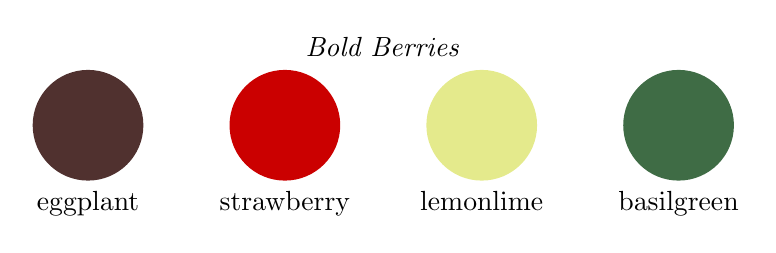
\begin{tikzpicture}[mynode/.style={circle,minimum size=40}]
\node at (6.25, 1) {\textit{Bold Berries}};
\definecolor{eggplant}{HTML}{50312F}
\definecolor{strawberry}{HTML}{CB0000}
\definecolor{lemonlime}{HTML}{E4EA8C}
\definecolor{basilgreen}{HTML}{3F6C45}
  \foreach \crlr/\pos in {eggplant/1,strawberry/2,lemonlime/3,basilgreen/4}
  {  \node [mynode,fill=\crlr,label=below:\crlr] () at (2.5*\pos,0) {};}
\end{tikzpicture}

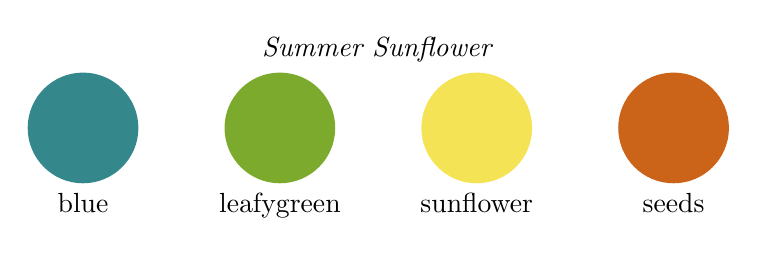
\begin{tikzpicture}[mynode/.style={circle,minimum size=40}]
\node at (6.25, 1) {\textit{Summer Sunflower}};
\definecolor{blue}{HTML}{34888C}
\definecolor{leafygreen}{HTML}{7CAA2D}
\definecolor{sunflower}{HTML}{F5E356}
\definecolor{seeds}{HTML}{CB6318}
  \foreach \crlr/\pos in {blue/1,leafygreen/2,sunflower/3,seeds/4}
  {  \node [mynode,fill=\crlr,label=below:\crlr] () at (2.5*\pos,0) {};}
\end{tikzpicture}

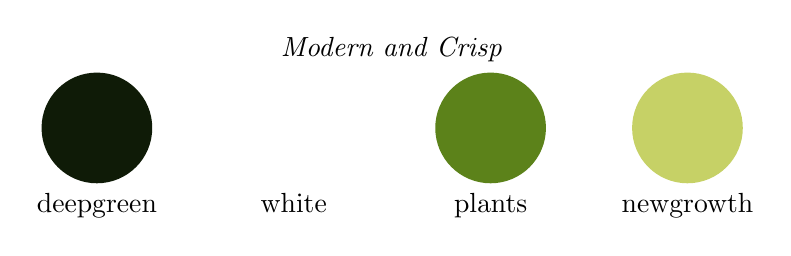
\begin{tikzpicture}[mynode/.style={circle,minimum size=40}]
\node at (6.25, 1) {\textit{Modern and Crisp}};
\definecolor{deepgreen}{HTML}{0F1B07}
\definecolor{white}{HTML}{FFFFFF}
\definecolor{plants}{HTML}{5C821A}
\definecolor{newgrowth}{HTML}{C6D166}
  \foreach \crlr/\pos in {deepgreen/1,white/2,plants/3,newgrowth/4}
  {  \node [mynode,fill=\crlr,label=below:\crlr] () at (2.5*\pos,0) {};}
\end{tikzpicture}

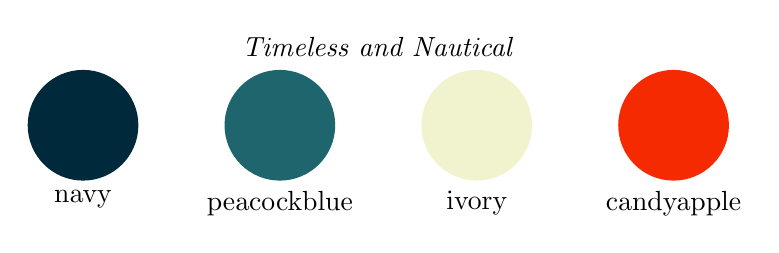
\begin{tikzpicture}[mynode/.style={circle,minimum size=40}]
\node at (6.25, 1) {\textit{Timeless and Nautical}};
\definecolor{navy}{HTML}{00293C}
\definecolor{peacockblue}{HTML}{1E656D}
\definecolor{ivory}{HTML}{F1F3CE}
\definecolor{candyapple}{HTML}{F62A00}
  \foreach \crlr/\pos in {navy/1,peacockblue/2,ivory/3,candyapple/4}
  {  \node [mynode,fill=\crlr,label=below:\crlr] () at (2.5*\pos,0) {};}
\end{tikzpicture}

% % % % % GROUP 26 - 30
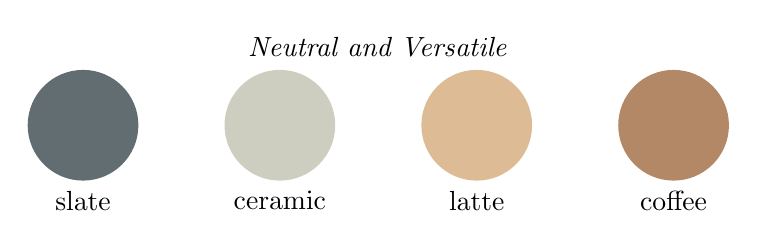
\begin{tikzpicture}[mynode/.style={circle,minimum size=40}]
\node at (6.25, 1) {\textit{Neutral and Versatile}};
\definecolor{slate}{HTML}{626D71}
\definecolor{ceramic}{HTML}{CDCDC0}
\definecolor{latte}{HTML}{DDBC95}
\definecolor{coffee}{HTML}{B38867}
  \foreach \crlr/\pos in {slate/1,ceramic/2,latte/3,coffee/4}
  {  \node [mynode,fill=\crlr,label=below:\crlr] () at (2.5*\pos,0) {};}
\end{tikzpicture}

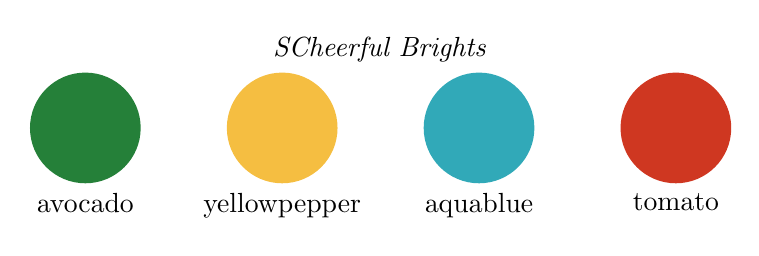
\begin{tikzpicture}[mynode/.style={circle,minimum size=40}]
\node at (6.25, 1) {\textit{SCheerful Brights}};
\definecolor{avocado}{HTML}{258039}
\definecolor{yellowpepper}{HTML}{F5BE41}
\definecolor{aquablue}{HTML}{31A9B8}
\definecolor{tomato}{HTML}{CF3721}
  \foreach \crlr/\pos in {avocado/1,yellowpepper/2,aquablue/3,tomato/4}
  {  \node [mynode,fill=\crlr,label=below:\crlr] () at (2.5*\pos,0) {};}
\end{tikzpicture}

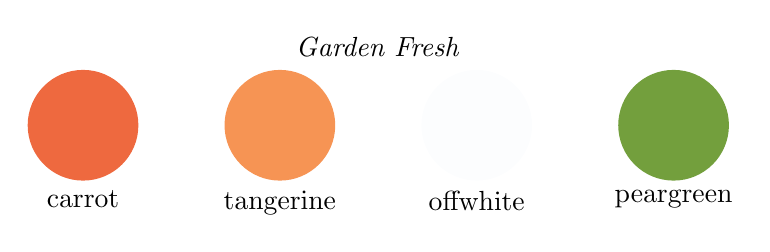
\begin{tikzpicture}[mynode/.style={circle,minimum size=40}]
\node at (6.25, 1) {\textit{Garden Fresh}};
\definecolor{carrot}{HTML}{EE693F}
\definecolor{tangerine}{HTML}{F69454}
\definecolor{offwhite}{HTML}{FCFDFE}
\definecolor{peargreen}{HTML}{739F3D}
  \foreach \crlr/\pos in {carrot/1,tangerine/2,offwhite/3,peargreen/4}
  {  \node [mynode,fill=\crlr,label=below:\crlr] () at (2.5*\pos,0) {};}
\end{tikzpicture}

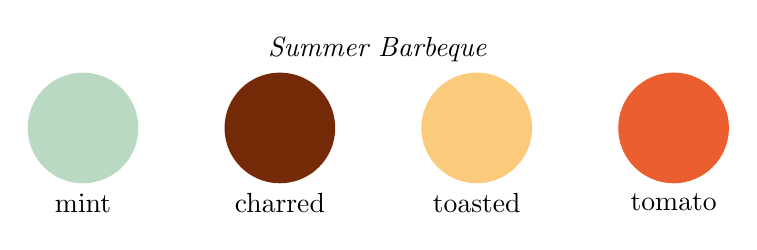
\begin{tikzpicture}[mynode/.style={circle,minimum size=40}]
\node at (6.25, 1) {\textit{Summer Barbeque}};
\definecolor{mint}{HTML}{B9D9C3}
\definecolor{charred}{HTML}{752A07}
\definecolor{toasted}{HTML}{FBCB7B}
\definecolor{tomato}{HTML}{EB5E30}
  \foreach \crlr/\pos in {mint/1,charred/2,toasted/3,tomato/4}
  {  \node [mynode,fill=\crlr,label=below:\crlr] () at (2.5*\pos,0) {};}
\end{tikzpicture}

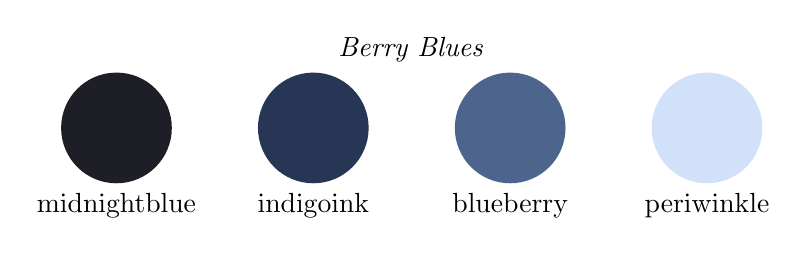
\begin{tikzpicture}[mynode/.style={circle,minimum size=40}]
\node at (6.25, 1) {\textit{Berry Blues}};
\definecolor{midnightblue}{HTML}{1E1F26}
\definecolor{indigoink}{HTML}{283655}
\definecolor{blueberry}{HTML}{4D648D}
\definecolor{periwinkle}{HTML}{D0E1F9}
  \foreach \crlr/\pos in {midnightblue/1,indigoink/2,blueberry/3,periwinkle/4}
  {  \node [mynode,fill=\crlr,label=below:\crlr] () at (2.5*\pos,0) {};}
\end{tikzpicture}

% % % % % GROUP 31 - 35
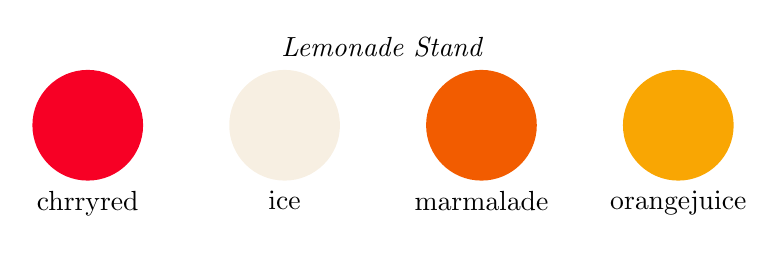
\begin{tikzpicture}[mynode/.style={circle,minimum size=40}]
\node at (6.25, 1) {\textit{Lemonade Stand}};
\definecolor{chrryred}{HTML}{F70025}
\definecolor{ice}{HTML}{F7EFE2}
\definecolor{marmalade}{HTML}{F25C00}
\definecolor{orangejuice}{HTML}{F9A603}
  \foreach \crlr/\pos in {chrryred/1,ice/2,marmalade/3,orangejuice/4}
  {  \node [mynode,fill=\crlr,label=below:\crlr] () at (2.5*\pos,0) {};}
\end{tikzpicture}

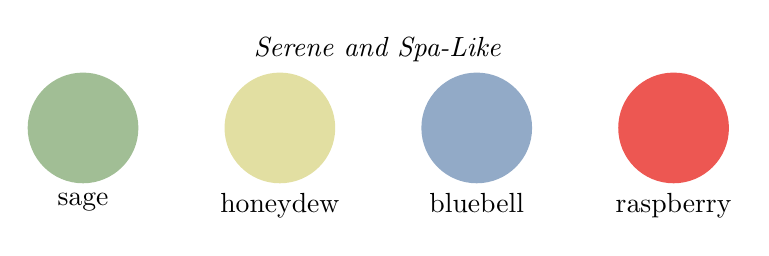
\begin{tikzpicture}[mynode/.style={circle,minimum size=40}]
\node at (6.25, 1) {\textit{Serene and Spa-Like}};
\definecolor{sage}{HTML}{A1BE95}
\definecolor{honeydew}{HTML}{E2DFA2}
\definecolor{bluebell}{HTML}{92AAC7}
\definecolor{raspberry}{HTML}{ED5752}
  \foreach \crlr/\pos in {sage/1,honeydew/2,bluebell/3,raspberry/4}
  {  \node [mynode,fill=\crlr,label=below:\crlr] () at (2.5*\pos,0) {};}
\end{tikzpicture}

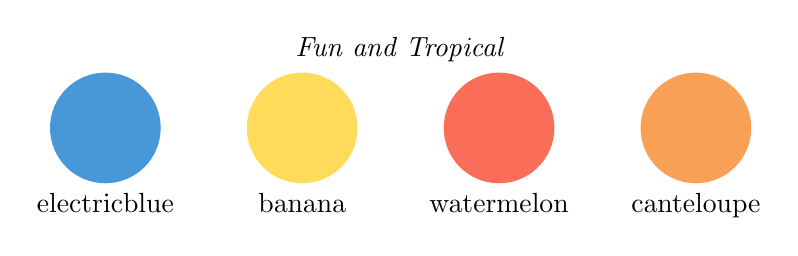
\begin{tikzpicture}[mynode/.style={circle,minimum size=40}]
\node at (6.25, 1) {\textit{Fun and Tropical}};
\definecolor{electricblue}{HTML}{4897D8}
\definecolor{banana}{HTML}{FFDB5C}
\definecolor{watermelon}{HTML}{FA6E59}
\definecolor{canteloupe}{HTML}{F8A055}
  \foreach \crlr/\pos in {electricblue/1,banana/2,watermelon/3,canteloupe/4}
  {  \node [mynode,fill=\crlr,label=below:\crlr] () at (2.5*\pos,0) {};}
\end{tikzpicture}

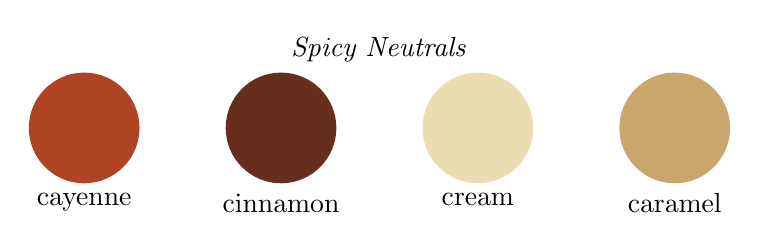
\begin{tikzpicture}[mynode/.style={circle,minimum size=40}]
\node at (6.25, 1) {\textit{Spicy Neutrals}};
\definecolor{cayenne}{HTML}{AF4425}
\definecolor{cinnamon}{HTML}{662E1C}
\definecolor{cream}{HTML}{EBDCB2}
\definecolor{caramel}{HTML}{C9A66B}
  \foreach \crlr/\pos in {cayenne/1,cinnamon/2,cream/3,caramel/4}
  {  \node [mynode,fill=\crlr,label=below:\crlr] () at (2.5*\pos,0) {};}
\end{tikzpicture}

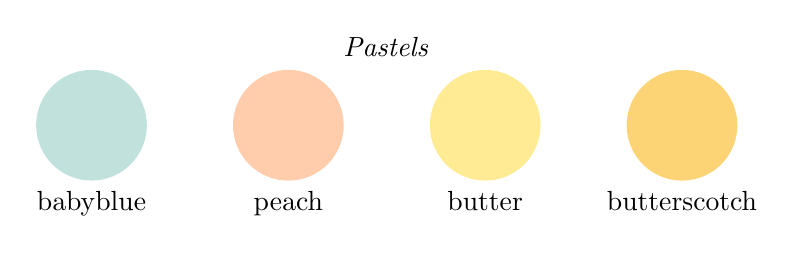
\begin{tikzpicture}[mynode/.style={circle,minimum size=40}]
\node at (6.25, 1) {\textit{Pastels}};
\definecolor{babyblue}{HTML}{C1E1DC}
\definecolor{peach}{HTML}{FFCCAC}
\definecolor{butter}{HTML}{FFEB94}
\definecolor{butterscotch}{HTML}{FDD475}
  \foreach \crlr/\pos in {babyblue/1,peach/2,butter/3,butterscotch/4}
  {  \node [mynode,fill=\crlr,label=below:\crlr] () at (2.5*\pos,0) {};}
\end{tikzpicture}

% % % % % GROUP 36 - 40
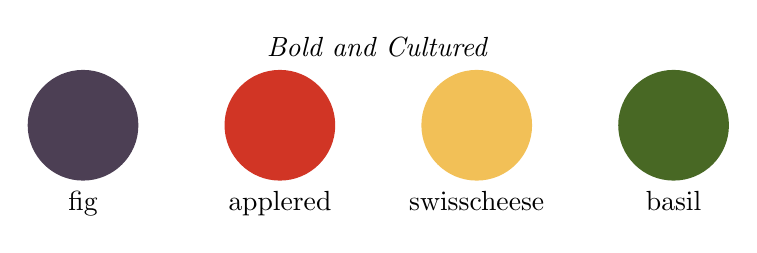
\begin{tikzpicture}[mynode/.style={circle,minimum size=40}]
\node at (6.25, 1) {\textit{Bold and Cultured}};
\definecolor{fig}{HTML}{4C3F54}
\definecolor{applered}{HTML}{D13525}
\definecolor{swisscheese}{HTML}{F2C057}
\definecolor{basil}{HTML}{486824}
  \foreach \crlr/\pos in {fig/1,applered/2,swisscheese/3,basil/4}
  {  \node [mynode,fill=\crlr,label=below:\crlr] () at (2.5*\pos,0) {};}
\end{tikzpicture}

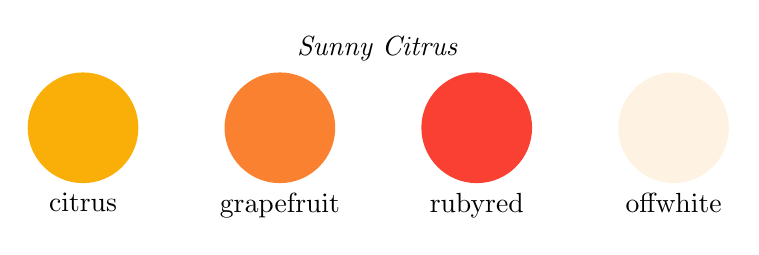
\begin{tikzpicture}[mynode/.style={circle,minimum size=40}]
\node at (6.25, 1) {\textit{Sunny Citrus}};
\definecolor{citrus}{HTML}{FAAF08}
\definecolor{grapefruit}{HTML}{FA812F}
\definecolor{rubyred}{HTML}{FA4032}
\definecolor{offwhite}{HTML}{FEF3E2}
  \foreach \crlr/\pos in {citrus/1,grapefruit/2,rubyred/3,offwhite/4}
  {  \node [mynode,fill=\crlr,label=below:\crlr] () at (2.5*\pos,0) {};}
\end{tikzpicture}

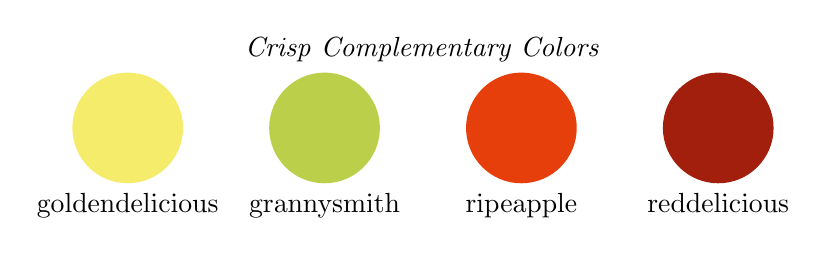
\begin{tikzpicture}[mynode/.style={circle,minimum size=40}]
\node at (6.25, 1) {\textit{Crisp Complementary Colors}};
\definecolor{goldendelicious}{HTML}{F4EC6A}
\definecolor{grannysmith}{HTML}{BBCF4A}
\definecolor{ripeapple}{HTML}{E73F0B}
\definecolor{reddelicious}{HTML}{A11F0C}
  \foreach \crlr/\pos in {goldendelicious/1,grannysmith/2,ripeapple/3,reddelicious/4}
  {  \node [mynode,fill=\crlr,label=below:\crlr] () at (2.5*\pos,0) {};}
\end{tikzpicture}

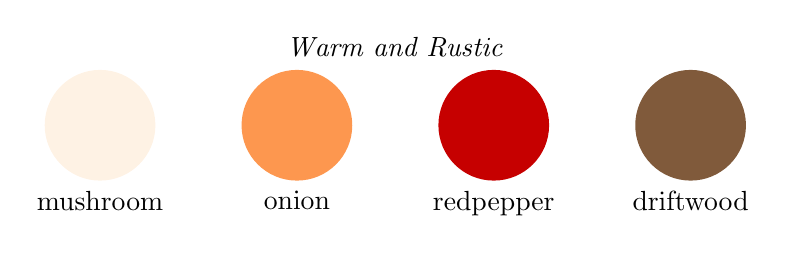
\begin{tikzpicture}[mynode/.style={circle,minimum size=40}]
\node at (6.25, 1) {\textit{Warm and Rustic}};
\definecolor{mushroom}{HTML}{FEF2E4}
\definecolor{onion}{HTML}{FD974F}
\definecolor{redpepper}{HTML}{C60000}
\definecolor{driftwood}{HTML}{805A3B}
  \foreach \crlr/\pos in {mushroom/1,onion/2,redpepper/3,driftwood/4}
  {  \node [mynode,fill=\crlr,label=below:\crlr] () at (2.5*\pos,0) {};}
\end{tikzpicture}

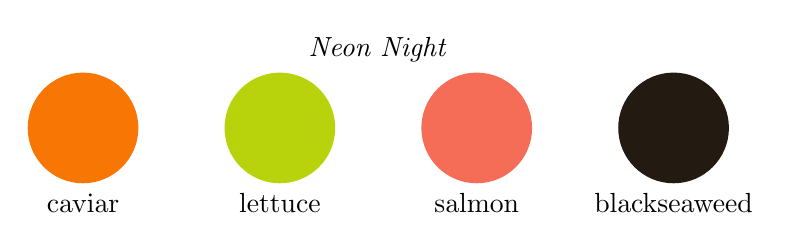
\begin{tikzpicture}[mynode/.style={circle,minimum size=40}]
\node at (6.25, 1) {\textit{Neon Night}};
\definecolor{caviar}{HTML}{F77604}
\definecolor{lettuce}{HTML}{B8D20B}
\definecolor{salmon}{HTML}{F56C57}
\definecolor{blackseaweed}{HTML}{231B12}
  \foreach \crlr/\pos in {caviar/1,lettuce/2,salmon/3,blackseaweed/4}
  {  \node [mynode,fill=\crlr,label=below:\crlr] () at (2.5*\pos,0) {};}
\end{tikzpicture}

% % % % % GROUP 41 - 45
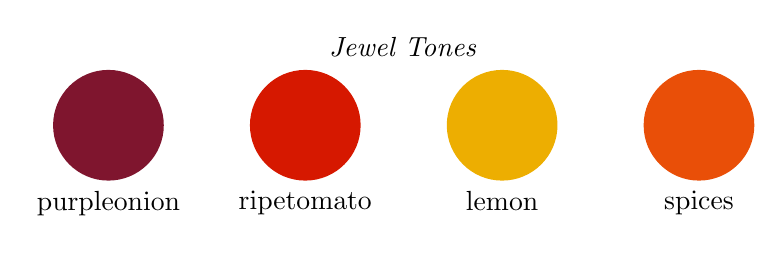
\begin{tikzpicture}[mynode/.style={circle,minimum size=40}]
\node at (6.25, 1) {\textit{Jewel Tones}};
\definecolor{purpleonion}{HTML}{7F152E}
\definecolor{ripetomato}{HTML}{D61800}
\definecolor{lemon}{HTML}{EDAE01}
\definecolor{spices}{HTML}{E94F08}
  \foreach \crlr/\pos in {purpleonion/1,ripetomato/2,lemon/3,spices/4}
  {  \node [mynode,fill=\crlr,label=below:\crlr] () at (2.5*\pos,0) {};}
\end{tikzpicture}

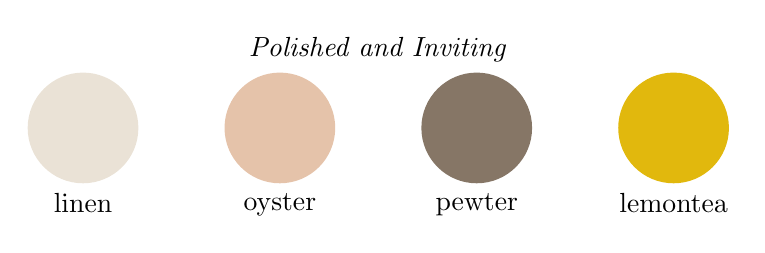
\begin{tikzpicture}[mynode/.style={circle,minimum size=40}]
\node at (6.25, 1) {\textit{Polished and Inviting}};
\definecolor{linen}{HTML}{EAE2D6}
\definecolor{oyster}{HTML}{E5C3AA}
\definecolor{pewter}{HTML}{867666}
\definecolor{lemontea}{HTML}{E1B80D}
  \foreach \crlr/\pos in {linen/1,oyster/2,pewter/3,lemontea/4}
  {  \node [mynode,fill=\crlr,label=below:\crlr] () at (2.5*\pos,0) {};}
\end{tikzpicture}

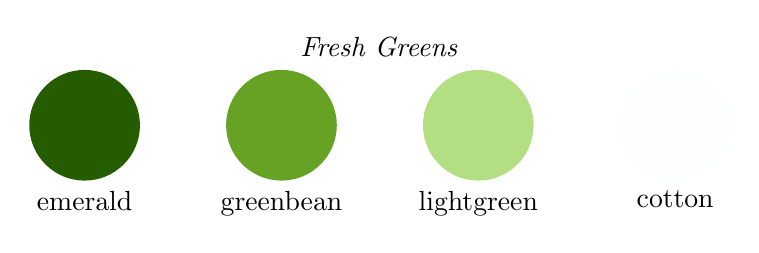
\begin{tikzpicture}[mynode/.style={circle,minimum size=40}]
\node at (6.25, 1) {\textit{Fresh Greens}};
\definecolor{emerald}{HTML}{265C00}
\definecolor{greenbean}{HTML}{68A225}
\definecolor{lightgreen}{HTML}{B3DE81}
\definecolor{cotton}{HTML}{FDFFFF}
  \foreach \crlr/\pos in {emerald/1,greenbean/2,lightgreen/3,cotton/4}
  {  \node [mynode,fill=\crlr,label=below:\crlr] () at (2.5*\pos,0) {};}
\end{tikzpicture}

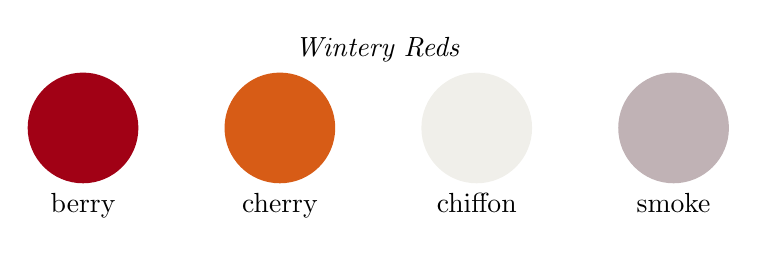
\begin{tikzpicture}[mynode/.style={circle,minimum size=40}]
\node at (6.25, 1) {\textit{Wintery Reds}};
\definecolor{berry}{HTML}{A10115}
\definecolor{cherry}{HTML}{D75C16}
\definecolor{chiffon}{HTML}{F0EFEA}
\definecolor{smoke}{HTML}{C0B2B5}
  \foreach \crlr/\pos in {berry/1,cherry/2,chiffon/3,smoke/4}
  {  \node [mynode,fill=\crlr,label=below:\crlr] () at (2.5*\pos,0) {};}
\end{tikzpicture}

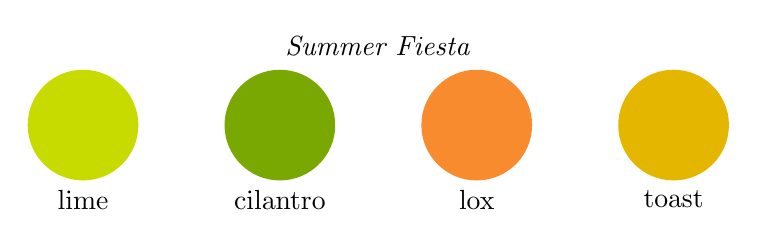
\begin{tikzpicture}[mynode/.style={circle,minimum size=40}]
\node at (6.25, 1) {\textit{Summer Fiesta}};
\definecolor{lime}{HTML}{C7DB00}
\definecolor{cilantro}{HTML}{7AA802}
\definecolor{lox}{HTML}{F78B2D}
\definecolor{toast}{HTML}{E4B600}
  \foreach \crlr/\pos in {lime/1,cilantro/2,lox/3,toast/4}
  {  \node [mynode,fill=\crlr,label=below:\crlr] () at (2.5*\pos,0) {};}
\end{tikzpicture}

% % % % % GROUP 46 - 50
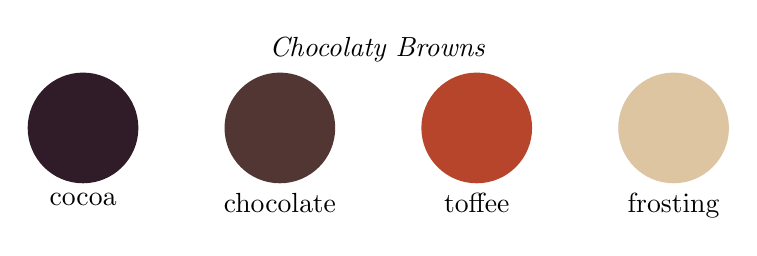
\begin{tikzpicture}[mynode/.style={circle,minimum size=40}]
\node at (6.25, 1) {\textit{Chocolaty Browns}};
\definecolor{cocoa}{HTML}{301B28}
\definecolor{chocolate}{HTML}{523634}
\definecolor{toffee}{HTML}{B6452C}
\definecolor{frosting}{HTML}{DDC5A2}
  \foreach \crlr/\pos in {cocoa/1,chocolate/2,toffee/3,frosting/4}
  {  \node [mynode,fill=\crlr,label=below:\crlr] () at (2.5*\pos,0) {};}
\end{tikzpicture}

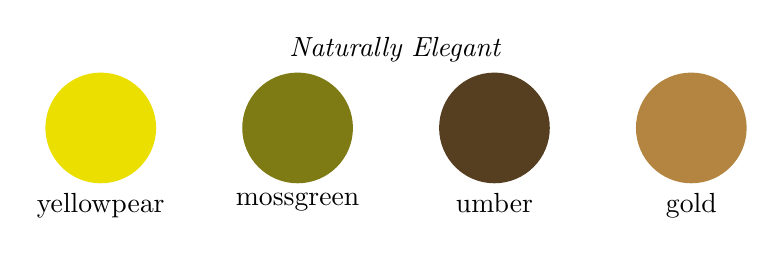
\begin{tikzpicture}[mynode/.style={circle,minimum size=40}]
\node at (6.25, 1) {\textit{Naturally Elegant}};
\definecolor{yellowpear}{HTML}{EBDF00}
\definecolor{mossgreen}{HTML}{7E7B15}
\definecolor{umber}{HTML}{563E20}
\definecolor{gold}{HTML}{B38540}
  \foreach \crlr/\pos in {yellowpear/1,mossgreen/2,umber/3,gold/4}
  {  \node [mynode,fill=\crlr,label=below:\crlr] () at (2.5*\pos,0) {};}
\end{tikzpicture}

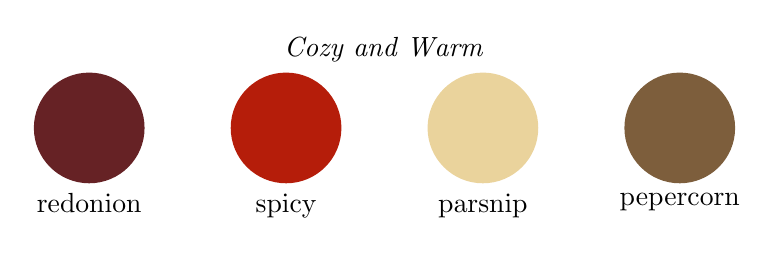
\begin{tikzpicture}[mynode/.style={circle,minimum size=40}]
\node at (6.25, 1) {\textit{Cozy and Warm}};
\definecolor{redonion}{HTML}{662225}
\definecolor{spicy}{HTML}{B51D0A}
\definecolor{parsnip}{HTML}{EAD39C}
\definecolor{pepercorn}{HTML}{7D5E3C}
  \foreach \crlr/\pos in {redonion/1,spicy/2,parsnip/3,pepercorn/4}
  {  \node [mynode,fill=\crlr,label=below:\crlr] () at (2.5*\pos,0) {};}
\end{tikzpicture}

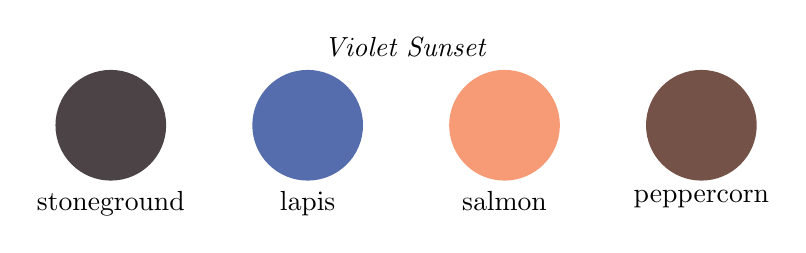
\begin{tikzpicture}[mynode/.style={circle,minimum size=40}]
\node at (6.25, 1) {\textit{Violet Sunset}};
\definecolor{stoneground}{HTML}{4B4345}
\definecolor{lapis}{HTML}{556DAC}
\definecolor{salmon}{HTML}{F79B77}
\definecolor{peppercorn}{HTML}{755248}
  \foreach \crlr/\pos in {stoneground/1,lapis/2,salmon/3,peppercorn/4}
  {  \node [mynode,fill=\crlr,label=below:\crlr] () at (2.5*\pos,0) {};}
\end{tikzpicture}

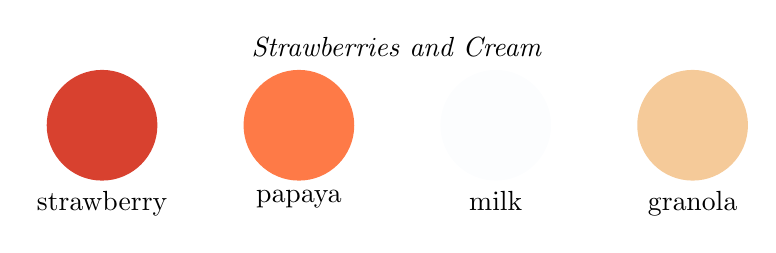
\begin{tikzpicture}[mynode/.style={circle,minimum size=40}]
\node at (6.25, 1) {\textit{Strawberries and Cream}};
\definecolor{strawberry}{HTML}{D8412F}
\definecolor{papaya}{HTML}{FE7A47}
\definecolor{milk}{HTML}{FCFDFE}
\definecolor{granola}{HTML}{F5CA99}
  \foreach \crlr/\pos in {strawberry/1,papaya/2,milk/3,granola/4}
  {  \node [mynode,fill=\crlr,label=below:\crlr] () at (2.5*\pos,0) {};}
\end{tikzpicture}

% % % % % GROUP 51 - 55
\begin{tikzpicture}[mynode/.style={circle,minimum size=40}]
\node at (6.25, 1) {\textit{Grecian Holiday}};
\definecolor{grecianblue}{HTML}{2988BC}
\definecolor{sea}{HTML}{2F496E}
\definecolor{plaster}{HTML}{F4EADE}
\definecolor{coral}{HTML}{ED8C72}
  \foreach \crlr/\pos in {grecianblue/1,sea/2,plaster/3,coral/4}
  {  \node [mynode,fill=\crlr,label=below:\crlr] () at (2.5*\pos,0) {};}
\end{tikzpicture}

\begin{tikzpicture}[mynode/.style={circle,minimum size=40}]
\node at (6.25, 1) {\textit{Bold and Basic}};
\definecolor{night}{HTML}{000B29}
\definecolor{phoneboothred}{HTML}{D70026}
\definecolor{pearl}{HTML}{F8F5F2}
\definecolor{flash}{HTML}{EDB83D}
  \foreach \crlr/\pos in {night/1,phoneboothred/2,pearl/3,flash/4}
  {  \node [mynode,fill=\crlr,label=below:\crlr] () at (2.5*\pos,0) {};}
\end{tikzpicture}

\begin{tikzpicture}[mynode/.style={circle,minimum size=40}]
\node at (6.25, 1) {\textit{Vineyard Neutrals}};
\definecolor{dark}{HTML}{1E0000}
\definecolor{wine}{HTML}{600906}
\definecolor{clay}{HTML}{9D331F}
\definecolor{dustyrose}{HTML}{BC6D4F}
  \foreach \crlr/\pos in {dark/1,wine/2,clay/3,dustyrose/4}
  {  \node [mynode,fill=\crlr,label=below:\crlr] () at (2.5*\pos,0) {};}
\end{tikzpicture}

\begin{tikzpicture}[mynode/.style={circle,minimum size=40}]
\node at (6.25, 1) {\textit{Modern and Urban}};
\definecolor{sunshine}{HTML}{F9BA32}
\definecolor{steelblue}{HTML}{426E86}
\definecolor{bone}{HTML}{F8F1E5}
\definecolor{coal}{HTML}{2F3131}
  \foreach \crlr/\pos in {sunshine/1,steelblue/2,bone/3,coal/4}
  {  \node [mynode,fill=\crlr,label=below:\crlr] () at (2.5*\pos,0) {};}
\end{tikzpicture}

\begin{tikzpicture}[mynode/.style={circle,minimum size=40}]
\node at (6.25, 1) {\textit{Misty Greens}};
\definecolor{forest}{HTML}{04202C}
\definecolor{evergreen}{HTML}{304040}
\definecolor{pine}{HTML}{5B7065}
\definecolor{fog}{HTML}{C9D1C8}
  \foreach \crlr/\pos in {forest/1,evergreen/2,pine/3,fog/4}
  {  \node [mynode,fill=\crlr,label=below:\crlr] () at (2.5*\pos,0) {};}
\end{tikzpicture}

% % % % % GROUP 56 - 60
\begin{tikzpicture}[mynode/.style={circle,minimum size=40}]
\node at (6.25, 1) {\textit{Sunkissed Village}};
\definecolor{terracotta}{HTML}{D24136}
\definecolor{honey}{HTML}{EB8A3E}
\definecolor{biscotti}{HTML}{EBB582}
\definecolor{stone}{HTML}{785A46}
  \foreach \crlr/\pos in {terracotta/1,honey/2,biscotti/3,stone/4}
  {  \node [mynode,fill=\crlr,label=below:\crlr] () at (2.5*\pos,0) {};}
\end{tikzpicture}

\begin{tikzpicture}[mynode/.style={circle,minimum size=40}]
\node at (6.25, 1) {\textit{Sun and Sky}};
\definecolor{ceruleanblue}{HTML}{217CA3}
\definecolor{mustard}{HTML}{E29930}
\definecolor{asphalt}{HTML}{32384D}
\definecolor{shadow}{HTML}{211F30}
  \foreach \crlr/\pos in {ceruleanblue/1,mustard/2,asphalt/3,shadow/4}
  {  \node [mynode,fill=\crlr,label=below:\crlr] () at (2.5*\pos,0) {};}
\end{tikzpicture}

\begin{tikzpicture}[mynode/.style={circle,minimum size=40}]
\node at (6.25, 1) {\textit{Aqua Blues}};
\definecolor{peacockblue}{HTML}{004D47}
\definecolor{deepaqua}{HTML}{128277}
\definecolor{lichen}{HTML}{52958B}
\definecolor{mist}{HTML}{B9C4C9}
  \foreach \crlr/\pos in {peacockblue/1,deepaqua/2,lichen/3,mist/4}
  {  \node [mynode,fill=\crlr,label=below:\crlr] () at (2.5*\pos,0) {};}
\end{tikzpicture}

\begin{tikzpicture}[mynode/.style={circle,minimum size=40}]
\node at (6.25, 1) {\textit{Urban Oasis}};
\definecolor{leaves}{HTML}{506D2F}
\definecolor{bark}{HTML}{2A2922}
\definecolor{marble}{HTML}{F3EBDD}
\definecolor{brownstone}{HTML}{7D5642}
  \foreach \crlr/\pos in {leaves/1,bark/2,marble/3,brownstone/4}
  {  \node [mynode,fill=\crlr,label=below:\crlr] () at (2.5*\pos,0) {};}
\end{tikzpicture}

\begin{tikzpicture}[mynode/.style={circle,minimum size=40}]
\node at (6.25, 1) {\textit{Candy-Coated Brights}};
\definecolor{orange}{HTML}{F47D4A}
\definecolor{fuschia}{HTML}{E1315B}
\definecolor{lemondrop}{HTML}{FFEC5C}
\definecolor{blueraspberry}{HTML}{008DCB}
  \foreach \crlr/\pos in {orange/1,fuschia/2,lemondrop/3,blueraspberry/4}
  {  \node [mynode,fill=\crlr,label=below:\crlr] () at (2.5*\pos,0) {};}
\end{tikzpicture}

% % % % % GROUP 61 - 65
\begin{tikzpicture}[mynode/.style={circle,minimum size=40}]
\node at (6.25, 1) {\textit{Muted and Antique}};
\definecolor{rubinseggblue}{HTML}{A4CABC}
\definecolor{nectar}{HTML}{EAB364}
\definecolor{tuscanred}{HTML}{B2473E}
\definecolor{olive}{HTML}{ACBD78}
  \foreach \crlr/\pos in {rubinseggblue/1,nectar/2,tuscanred/3,olive/4}
  {  \node [mynode,fill=\crlr,label=below:\crlr] () at (2.5*\pos,0) {};}
\end{tikzpicture}

\begin{tikzpicture}[mynode/.style={circle,minimum size=40}]
\node at (6.25, 1) {\textit{Classy and Timeless}};
\definecolor{midnightblue}{HTML}{16253D}
\definecolor{dusk}{HTML}{002C54}
\definecolor{golden}{HTML}{EFB509}
\definecolor{bronze}{HTML}{CD7213}
  \foreach \crlr/\pos in {midnightblue/1,dusk/2,golden/3,bronze/4}
  {  \node [mynode,fill=\crlr,label=below:\crlr] () at (2.5*\pos,0) {};}
\end{tikzpicture}

\begin{tikzpicture}[mynode/.style={circle,minimum size=40}]
\node at (6.25, 1) {\textit{Cosmopolitan}};
\definecolor{bluegray}{HTML}{8593AE}
\definecolor{steel}{HTML}{5A4E4D}
\definecolor{pewter}{HTML}{7E675E}
\definecolor{blush}{HTML}{DDA288}
  \foreach \crlr/\pos in {bluegray/1,steel/2,pewter/3,blush/4}
  {  \node [mynode,fill=\crlr,label=below:\crlr] () at (2.5*\pos,0) {};}
\end{tikzpicture}

\begin{tikzpicture}[mynode/.style={circle,minimum size=40}]
\node at (6.25, 1) {\textit{Cheerful and Friendly}};
\definecolor{darkteal}{HTML}{2B616D}
\definecolor{arctic}{HTML}{B2DBD5}
\definecolor{whitecloud}{HTML}{FFFFFF}
\definecolor{brick}{HTML}{FA8D62}
  \foreach \crlr/\pos in {darkteal/1,arctic/2,whitecloud/3,brick/4}
  {  \node [mynode,fill=\crlr,label=below:\crlr] () at (2.5*\pos,0) {};}
\end{tikzpicture}

\begin{tikzpicture}[mynode/.style={circle,minimum size=40}]
\node at (6.25, 1) {\textit{Nightlife}};
\definecolor{cyan}{HTML}{00CFFA}
\definecolor{magenta}{HTML}{FF0038}
\definecolor{yellow}{HTML}{FFCE38}
\definecolor{black}{HTML}{020509}
  \foreach \crlr/\pos in {cyan/1,magenta/2,yellow/3,black/4}
  {  \node [mynode,fill=\crlr,label=below:\crlr] () at (2.5*\pos,0) {};}
\end{tikzpicture}

% % % % % GROUP 66 - 70
\begin{tikzpicture}[mynode/.style={circle,minimum size=40}]
\node at (6.25, 1) {\textit{Coastal}};
\definecolor{powder}{HTML}{A5C3CF}
\definecolor{clouds}{HTML}{F3D3B8}
\definecolor{sand}{HTML}{E59D5C}
\definecolor{palm}{HTML}{A99F3C}
  \foreach \crlr/\pos in {powder/1,clouds/2,sand/3,palm/4}
  {  \node [mynode,fill=\crlr,label=below:\crlr] () at (2.5*\pos,0) {};}
\end{tikzpicture}

\begin{tikzpicture}[mynode/.style={circle,minimum size=40}]
\node at (6.25, 1) {\textit{Maritime Brights}};
\definecolor{saltwater}{HTML}{257985}
\definecolor{lagoon}{HTML}{5EA8A7}
\definecolor{whitewash}{HTML}{FFFFFF}
\definecolor{raspberry}{HTML}{FF4447}
  \foreach \crlr/\pos in {saltwater/1,lagoon/2,whitewash/3,raspberry/4}
  {  \node [mynode,fill=\crlr,label=below:\crlr] () at (2.5*\pos,0) {};}
\end{tikzpicture}

\begin{tikzpicture}[mynode/.style={circle,minimum size=40}]
\node at (6.25, 1) {\textit{Vintage Charm}};
\definecolor{honeysuckle}{HTML}{FCC875}
\definecolor{warmgray}{HTML}{BAA896}
\definecolor{putty}{HTML}{E6CCB5}
\definecolor{fadedrose}{HTML}{E38B75}
  \foreach \crlr/\pos in {honeysuckle/1,warmgray/2,putty/3,fadedrose/4}
  {  \node [mynode,fill=\crlr,label=below:\crlr] () at (2.5*\pos,0) {};}
\end{tikzpicture}

\begin{tikzpicture}[mynode/.style={circle,minimum size=40}]
\node at (6.25, 1) {\textit{Understated and Versatile}};
\definecolor{stormysea}{HTML}{335252}
\definecolor{fog}{HTML}{D4DDE1}
\definecolor{rust}{HTML}{AA4B41}
\definecolor{charcoal}{HTML}{2D3033}
  \foreach \crlr/\pos in {stormysea/1,fog/2,rust/3,charcoal/4}
  {  \node [mynode,fill=\crlr,label=below:\crlr] () at (2.5*\pos,0) {};}
\end{tikzpicture}

\begin{tikzpicture}[mynode/.style={circle,minimum size=40}]
\node at (6.25, 1) {\textit{Arctic Sunrise}};
\definecolor{sunrise}{HTML}{FFCCBB}
\definecolor{bluetopaz}{HTML}{6EB5C0}
\definecolor{cerulean}{HTML}{006C84}
\definecolor{icicle}{HTML}{E2E8E4}
  \foreach \crlr/\pos in {sunrise/1,bluetopaz/2,cerulean/3,icicle/4}
  {  \node [mynode,fill=\crlr,label=below:\crlr] () at (2.5*\pos,0) {};}
\end{tikzpicture}

% % % % % GROUP 71 - 75
\begin{tikzpicture}[mynode/.style={circle,minimum size=40}]
\node at (6.25, 1) {\textit{Mediterranean Afternoon}};
\definecolor{currant}{HTML}{8C0004}
\definecolor{scarlet}{HTML}{C8000A}
\definecolor{marigold}{HTML}{E8A735}
\definecolor{cobblestone}{HTML}{E2C499}
  \foreach \crlr/\pos in {currant/1,scarlet/2,marigold/3,cobblestone/4}
  {  \node [mynode,fill=\crlr,label=below:\crlr] () at (2.5*\pos,0) {};}
\end{tikzpicture}

\begin{tikzpicture}[mynode/.style={circle,minimum size=40}]
\node at (6.25, 1) {\textit{Hazy Grays}};
\definecolor{bluegreen}{HTML}{2C4A52}
\definecolor{waterway}{HTML}{537072}
\definecolor{haze}{HTML}{8E9B97}
\definecolor{smog}{HTML}{F4EBDB}
  \foreach \crlr/\pos in {bluegreen/1,waterway/2,haze/3,smog/4}
  {  \node [mynode,fill=\crlr,label=below:\crlr] () at (2.5*\pos,0) {};}
\end{tikzpicture}

\begin{tikzpicture}[mynode/.style={circle,minimum size=40}]
\node at (6.25, 1) {\textit{City Sights}};
\definecolor{fireenginered}{HTML}{C5001A}
\definecolor{lightgray}{HTML}{E4E3DB}
\definecolor{denim}{HTML}{113743}
\definecolor{concrete}{HTML}{C5BEBA}
  \foreach \crlr/\pos in {fireenginered/1,lightgray/2,denim/3,concrete/4}
  {  \node [mynode,fill=\crlr,label=below:\crlr] () at (2.5*\pos,0) {};}
\end{tikzpicture}

\begin{tikzpicture}[mynode/.style={circle,minimum size=40}]
\node at (6.25, 1) {\textit{Retro and Relaxing}};
\definecolor{ginger}{HTML}{D35C37}
\definecolor{hazelnut}{HTML}{BF9A77}
\definecolor{oat}{HTML}{D6C6B9}
\definecolor{sky}{HTML}{97B8C2}
  \foreach \crlr/\pos in {ginger/1,hazelnut/2,oat/3,sky/4}
  {  \node [mynode,fill=\crlr,label=below:\crlr] () at (2.5*\pos,0) {};}
\end{tikzpicture}

\begin{tikzpicture}[mynode/.style={circle,minimum size=40}]
\node at (6.25, 1) {\textit{Green Fields}};
\definecolor{splitpea}{HTML}{919636}
\definecolor{camouflage}{HTML}{524A3A}
\definecolor{light}{HTML}{FFFAE1}
\definecolor{grass}{HTML}{5A5F37}
  \foreach \crlr/\pos in {splitpea/1,camouflage/2,light/3,grass/4}
  {  \node [mynode,fill=\crlr,label=below:\crlr] () at (2.5*\pos,0) {};}
\end{tikzpicture}

% % % % % GROUP 76 - 80
\begin{tikzpicture}[mynode/.style={circle,minimum size=40}]
\node at (6.25, 1) {\textit{Distinctive and Unexpected}};
\definecolor{turquoise}{HTML}{52908B}
\definecolor{coolgray}{HTML}{E5E2CA}
\definecolor{brownishpurple}{HTML}{DDBC95}
\definecolor{orangered}{HTML}{E7472E}
  \foreach \crlr/\pos in {turquoise/1,coolgray/2,brownishpurple/3,orangered/4}
  {  \node [mynode,fill=\crlr,label=below:\crlr] () at (2.5*\pos,0) {};}
\end{tikzpicture}

\begin{tikzpicture}[mynode/.style={circle,minimum size=40}]
\node at (6.25, 1) {\textit{Sleek and Modern}};
\definecolor{blueblack}{HTML}{2F2E33}
\definecolor{coolgray}{HTML}{D5D6D2}
\definecolor{white}{HTML}{FFFFFF}
\definecolor{cobalt}{HTML}{3A5199}
  \foreach \crlr/\pos in {blueblack/1,coolgray/2,white/3,cobalt/4}
  {  \node [mynode,fill=\crlr,label=below:\crlr] () at (2.5*\pos,0) {};}
\end{tikzpicture}

\begin{tikzpicture}[mynode/.style={circle,minimum size=40}]
\node at (6.25, 1) {\textit{Orange Accent}};
\definecolor{woodveneer}{HTML}{756867}
\definecolor{sanddollar}{HTML}{D5D6D2}
\definecolor{charcoal}{HTML}{353C3F}
\definecolor{orange}{HTML}{FF8D3F}
  \foreach \crlr/\pos in {woodveneer/1,sanddollar/2,charcoal/3,orange/4}
  {  \node [mynode,fill=\crlr,label=below:\crlr] () at (2.5*\pos,0) {};}
\end{tikzpicture}

\begin{tikzpicture}[mynode/.style={circle,minimum size=40}]
\node at (6.25, 1) {\textit{Beyond Black and White}};
\definecolor{turquoise}{HTML}{31A2AC}
\definecolor{lipstick}{HTML}{AF1C1C}
\definecolor{grayishwhite}{HTML}{F0EFF0}
\definecolor{oldwood}{HTML}{2F2F28}
  \foreach \crlr/\pos in {turquoise/1,lipstick/2,grayishwhite/3,oldwood/4}
  {  \node [mynode,fill=\crlr,label=below:\crlr] () at (2.5*\pos,0) {};}
\end{tikzpicture}

\begin{tikzpicture}[mynode/.style={circle,minimum size=40}]
\node at (6.25, 1) {\textit{Shabby Chic Neutrals}};
\definecolor{metal}{HTML}{6C5F5B}
\definecolor{kragtpaper}{HTML}{CDAB81}
\definecolor{newsprint}{HTML}{DAC3B3}
\definecolor{pewter}{HTML}{4F4A45}
  \foreach \crlr/\pos in {metal/1,kragtpaper/2,newsprint/3,pewter/4}
  {  \node [mynode,fill=\crlr,label=below:\crlr] () at (2.5*\pos,0) {};}
\end{tikzpicture}

% % % % % GROUP 81 - 85
\begin{tikzpicture}[mynode/.style={circle,minimum size=40}]
\node at (6.25, 1) {\textit{Warm and Cool}};
\definecolor{fadednavy}{HTML}{444C5C}
\definecolor{punch}{HTML}{CE5A57}
\definecolor{oceanbreeze}{HTML}{78A5A3}
\definecolor{warm}{HTML}{E1B16A}
  \foreach \crlr/\pos in {fadednavy/1,punch/2,oceanbreeze/3,warm/4}
  {  \node [mynode,fill=\crlr,label=below:\crlr] () at (2.5*\pos,0) {};}
\end{tikzpicture}

\begin{tikzpicture}[mynode/.style={circle,minimum size=40}]
\node at (6.25, 1) {\textit{Industrial and In-Control}};
\definecolor{ink}{HTML}{20232A}
\definecolor{aluminum}{HTML}{ACBEBE}
\definecolor{paper}{HTML}{F4F4EF}
\definecolor{rubyred}{HTML}{A01D26}
  \foreach \crlr/\pos in {ink/1,aluminum/2,paper/3,rubyred/4}
  {  \node [mynode,fill=\crlr,label=below:\crlr] () at (2.5*\pos,0) {};}
\end{tikzpicture}

\begin{tikzpicture}[mynode/.style={circle,minimum size=40}]
\node at (6.25, 1) {\textit{Autumn Oranges + Complementary Neutrals}};
\definecolor{pumpkin}{HTML}{D55448}
\definecolor{canteloupe}{HTML}{FFA577}
\definecolor{cotton}{HTML}{F9F9FF}
\definecolor{hotchocolate}{HTML}{896E69}
  \foreach \crlr/\pos in {pumpkin/1,canteloupe/2,cotton/3,hotchocolate/4}
  {  \node [mynode,fill=\crlr,label=below:\crlr] () at (2.5*\pos,0) {};}
\end{tikzpicture}

\begin{tikzpicture}[mynode/.style={circle,minimum size=40}]
\node at (6.25, 1) {\textit{Pool Party}};
\definecolor{royalblue}{HTML}{344D90}
\definecolor{poolblue}{HTML}{5CC5EF}
\definecolor{orangejuice}{HTML}{FFB745}
\definecolor{bloodorange}{HTML}{E7552C}
  \foreach \crlr/\pos in {royalblue/1,poolblue/2,orangejuice/3,bloodorange/4}
  {  \node [mynode,fill=\crlr,label=below:\crlr] () at (2.5*\pos,0) {};}
\end{tikzpicture}

\begin{tikzpicture}[mynode/.style={circle,minimum size=40}]
\node at (6.25, 1) {\textit{Classic Metallics}};
\definecolor{blacksteel}{HTML}{080706}
\definecolor{paper}{HTML}{EFEFEF}
\definecolor{goldleaf}{HTML}{D1B280}
\definecolor{silver}{HTML}{594D46}
  \foreach \crlr/\pos in {blacksteel/1,paper/2,goldleaf/3,silver/4}
  {  \node [mynode,fill=\crlr,label=below:\crlr] () at (2.5*\pos,0) {};}
\end{tikzpicture}

% % % % % GROUP 86 - 90
\begin{tikzpicture}[mynode/.style={circle,minimum size=40}]
\node at (6.25, 1) {\textit{Subtle and Versatile}};
\definecolor{bluegreen}{HTML}{5F968E}
\definecolor{minty}{HTML}{BFDCCF}
\definecolor{fadedred}{HTML}{E05858}
\definecolor{oatmeal}{HTML}{D5C9B1}
  \foreach \crlr/\pos in {bluegreen/1,minty/2,fadedred/3,oatmeal/4}
  {  \node [mynode,fill=\crlr,label=below:\crlr] () at (2.5*\pos,0) {};}
\end{tikzpicture}

\begin{tikzpicture}[mynode/.style={circle,minimum size=40}]
\node at (6.25, 1) {\textit{Professional and Traditional}};
\definecolor{brickred}{HTML}{962715}
\definecolor{glosswhite}{HTML}{FFFFFF}
\definecolor{matteblack}{HTML}{1E1E20}
\definecolor{mediumgray}{HTML}{BBC3C6}
  \foreach \crlr/\pos in {brickred/1,glosswhite/2,matteblack/3,mediumgray/4}
  {  \node [mynode,fill=\crlr,label=below:\crlr] () at (2.5*\pos,0) {};}
\end{tikzpicture}

\begin{tikzpicture}[mynode/.style={circle,minimum size=40}]
\node at (6.25, 1) {\textit{Light and Natural}};
\definecolor{stone}{HTML}{688B8A}
\definecolor{sage}{HTML}{A0B084}
\definecolor{buttermilk}{HTML}{FAEFD4}
\definecolor{leather}{HTML}{A57C65}
  \foreach \crlr/\pos in {stone/1,sage/2,buttermilk/3,leather/4}
  {  \node [mynode,fill=\crlr,label=below:\crlr] () at (2.5*\pos,0) {};}
\end{tikzpicture}

\begin{tikzpicture}[mynode/.style={circle,minimum size=40}]
\node at (6.25, 1) {\textit{Shadowy and Dramatic}};
\definecolor{slate}{HTML}{262F34}
\definecolor{neonred}{HTML}{F34A4A}
\definecolor{crepe}{HTML}{F1D3BC}
\definecolor{bownishgray}{HTML}{615049}
  \foreach \crlr/\pos in {slate/1,neonred/2,crepe/3,bownishgray/4}
  {  \node [mynode,fill=\crlr,label=below:\crlr] () at (2.5*\pos,0) {};}
\end{tikzpicture}

\begin{tikzpicture}[mynode/.style={circle,minimum size=40}]
\node at (6.25, 1) {\textit{Golden Afternoon}};
\definecolor{burgundy}{HTML}{882426}
\definecolor{sidewalk}{HTML}{CDBEA7}
\definecolor{cinder}{HTML}{323030}
\definecolor{goldenafternoon}{HTML}{C29545}
  \foreach \crlr/\pos in {burgundy/1,sidewalk/2,cinder/3,goldenafternoon/4}
  {  \node [mynode,fill=\crlr,label=below:\crlr] () at (2.5*\pos,0) {};}
\end{tikzpicture}

% % % % % GROUP 91 - 95
\begin{tikzpicture}[mynode/.style={circle,minimum size=40}]
\node at (6.25, 1) {\textit{Dark and Handsome}};
\definecolor{mahogany}{HTML}{42313A}
\definecolor{chestnut}{HTML}{6C2D2C}
\definecolor{leather}{HTML}{9F4636}
\definecolor{parchment}{HTML}{F1DCC9}
  \foreach \crlr/\pos in {mahogany/1,chestnut/2,leather/3,parchment/4}
  {  \node [mynode,fill=\crlr,label=below:\crlr] () at (2.5*\pos,0) {};}
\end{tikzpicture}

\begin{tikzpicture}[mynode/.style={circle,minimum size=40}]
\node at (6.25, 1) {\textit{Technology Meets Nature}};
\definecolor{buttercup}{HTML}{FBCD4B}
\definecolor{silverplate}{HTML}{A3A599}
\definecolor{dark}{HTML}{282623}
\definecolor{algae}{HTML}{88A550}
  \foreach \crlr/\pos in {buttercup/1,silverplate/2,dark/3,algae/4}
  {  \node [mynode,fill=\crlr,label=below:\crlr] () at (2.5*\pos,0) {};}
\end{tikzpicture}

\begin{tikzpicture}[mynode/.style={circle,minimum size=40}]
\node at (6.25, 1) {\textit{Cheerful Blues + Pink}};
\definecolor{softpink}{HTML}{FFBEBD}
\definecolor{warmwhite}{HTML}{FCFCFA}
\definecolor{brightblue}{HTML}{337BAE}
\definecolor{aegeanblue}{HTML}{1A405F}
  \foreach \crlr/\pos in {softpink/1,warmwhite/2,brightblue/3,aegeanblue/4}
  {  \node [mynode,fill=\crlr,label=below:\crlr] () at (2.5*\pos,0) {};}
\end{tikzpicture}

\begin{tikzpicture}[mynode/.style={circle,minimum size=40}]
\node at (6.25, 1) {\textit{Exotic and High-Impact}};
\definecolor{onyx}{HTML}{0F1F38}
\definecolor{taupe}{HTML}{8E7970}
\definecolor{firework}{HTML}{F55449}
\definecolor{oceanic}{HTML}{1B4B5A}
  \foreach \crlr/\pos in {onyx/1,taupe/2,firework/3,oceanic/4}
  {  \node [mynode,fill=\crlr,label=below:\crlr] () at (2.5*\pos,0) {};}
\end{tikzpicture}

\begin{tikzpicture}[mynode/.style={circle,minimum size=40}]
\node at (6.25, 1) {\textit{Back to School}};
\definecolor{wood}{HTML}{81715E}
\definecolor{pencilyellow}{HTML}{FAAE3D}
\definecolor{orange}{HTML}{E38533}
\definecolor{pinkeraser}{HTML}{E4535E}
  \foreach \crlr/\pos in {wood/1,pencilyellow/2,orange/3,pinkeraser/4}
  {  \node [mynode,fill=\crlr,label=below:\crlr] () at (2.5*\pos,0) {};}
\end{tikzpicture}

% % % % % GROUP 96 - 100
\begin{tikzpicture}[mynode/.style={circle,minimum size=40}]
\node at (6.25, 1) {\textit{Bright and Painterly}};
\definecolor{ultramarine}{HTML}{061283}
\definecolor{watermelon}{HTML}{FD3C3C}
\definecolor{sunshine}{HTML}{FFB74C}
\definecolor{turquoise}{HTML}{138D90}
  \foreach \crlr/\pos in {ultramarine/1,watermelon/2,sunshine/3,turquoise/4}
  {  \node [mynode,fill=\crlr,label=below:\crlr] () at (2.5*\pos,0) {};}
\end{tikzpicture}

\begin{tikzpicture}[mynode/.style={circle,minimum size=40}]
\node at (6.25, 1) {\textit{Urban Living}};
\definecolor{softgray}{HTML}{DDDEDE}
\definecolor{blackish}{HTML}{232122}
\definecolor{houseplant}{HTML}{A5C05B}
\definecolor{bluegray}{HTML}{7BA4A8}
  \foreach \crlr/\pos in {softgray/1,blackish/2,houseplant/3,bluegray/4}
  {  \node [mynode,fill=\crlr,label=below:\crlr] () at (2.5*\pos,0) {};}
\end{tikzpicture}

\begin{tikzpicture}[mynode/.style={circle,minimum size=40}]
\node at (6.25, 1) {\textit{1950s Kitchen}};
\definecolor{mint}{HTML}{B3DBC0}
\definecolor{red}{HTML}{FE0000}
\definecolor{porcelain}{HTML}{FDF6F6}
\definecolor{freshblue}{HTML}{67BACA}
  \foreach \crlr/\pos in {mint/1,red/2,porcelain/3,freshblue/4}
  {  \node [mynode,fill=\crlr,label=below:\crlr] () at (2.5*\pos,0) {};}
\end{tikzpicture}

\begin{tikzpicture}[mynode/.style={circle,minimum size=40}]
\node at (6.25, 1) {\textit{Smoky Purples}};
\definecolor{warmgray}{HTML}{A49592}
\definecolor{darbluishgray}{HTML}{727077}
\definecolor{beige}{HTML}{EED8C9}
\definecolor{mauve}{HTML}{E99787}
  \foreach \crlr/\pos in {warmgray/1,darbluishgray/2,beige/3,mauve/4}
  {  \node [mynode,fill=\crlr,label=below:\crlr] () at (2.5*\pos,0) {};}
\end{tikzpicture}

\begin{tikzpicture}[mynode/.style={circle,minimum size=40}]
\node at (6.25, 1) {\textit{Trendy and Metropolitan}};
\definecolor{darkaqua}{HTML}{488A99}
\definecolor{gold}{HTML}{DBAE58}
\definecolor{charcoal}{HTML}{FBE9E7}
\definecolor{gray}{HTML}{B4B4B4}
  \foreach \crlr/\pos in {darkaqua/1,gold/2,charcoal/3,gray/4}
  {  \node [mynode,fill=\crlr,label=below:\crlr] () at (2.5*\pos,0) {};}
\end{tikzpicture}















\end{document}

%\path [draw, -latex'] (CPM) -| (VMBM);
%\node[draw, circle] at (1,1) {$test$};
